\section{SIFT and SURF Descriptor}
\label{sec:build2}

\textbf{Speed up Robust Features(SURF) - } SURF is a high performance, fast scale and rotation invariant point detector and descriptor.The task of finding point correspondences between two images of the same scene or object is part of many computer vision applications. Image registration, camera calibration, object recognition, and image retrieval are just a few.The search for discrete image point correspondences can be divided into three main steps. First, ‘interest points’ are selected at distinctive locations in the image, such as corners, blobs, and T-junctions. The most valuable prop- erty of an interest point detector is its repeatability. The repeatability expresses the reliability of a detector for find- ing the same physical interest points under different viewing conditions. Next, the neighbourhood of every interest point is represented by a feature vector. This descriptor has to be distinctive and at the same time robust to noise, de- tection displacements and geometric and photometric deformations. Finally, the descriptor vectors are matched be- tween different images. The matching is based on a distance between the vectors, e.g. the Mahalanobis or Euclidean distance. The dimension of the descriptor has a direct impact on the time this takes, and less dimensions are desirable for fast interest point matching. However, lower dimensional feature vectors are in general less distinctive than their high-dimensional counterparts.
It has been our goal to develop both a detector and de- scriptor that, in comparison to the state-of-the-art, are fast to compute while not sacrificing performance. In order to succeed, one has to strike a balance between the above requirements like simplifying the detection scheme while keeping it accurate, and reducing the descriptor’s size while keeping it sufficiently distinctive.
 It outperforms previously proposed schemes with respect to repeatability, distinctiveness and robustness [9]. The detector is based on the Hessian matrix and uses a very basic Laplacian-based detector, called difference of Gaussian (DoG). The implementation of SURF can be divided into three main steps. First, interest points are selected at distinctive locations in the image, such as corners, blobs, and T-junctions. Then, the neighborhood of every interest point is represented by a feature vector. This descriptor has to be distinctive and robust to noise, detection errors, and geometric and photometric deformations. Finally, the descriptor vectors are matched between different images. When working with local features, the issue that needs to be settled is the required level of invariance. Here the rotation and scale invariant descriptors seem to offer a good compromise between feature complexity and robustness to commonly occurring deformations, skew, anisotropic scaling, and perspective effects [9].

Given a point in an Image, the Hessian matrix is as follows:

\[
H(x,\sigma) =  
	\begin{bmatrix}
		L_{xx}(x,\sigma) &  L_{xy}(x,\sigma)\\
		L_{xy}(x,\sigma) &  L_{yy}(x,\sigma)
	\end{bmatrix}
\]

where $L_{xx}(x,\sigma)$ is the convolution of the gaussian second order derivative 
$\frac{d^2}{dy^2}g(\sigma)$ at the point. This method leads to a novel detection, description and subsequent matching steps. Using relative strengths and orientations of gradient reduces the effect of photometric changes. Figure \ref{fig:Figure9} shows the detection results with respect to rotation and scale change. As shown in Section 4, it has been found that though SURF is rotation invariant, its performance in matching, i.e. matching score, decreases sharply when the im- ages are rotated or scaled. The SURF features are not stable over various rotation angles and scale changes.
\\ 
\begin{figure}
	\DeclareGraphicsExtensions{.pdf,.png,.jpg}
	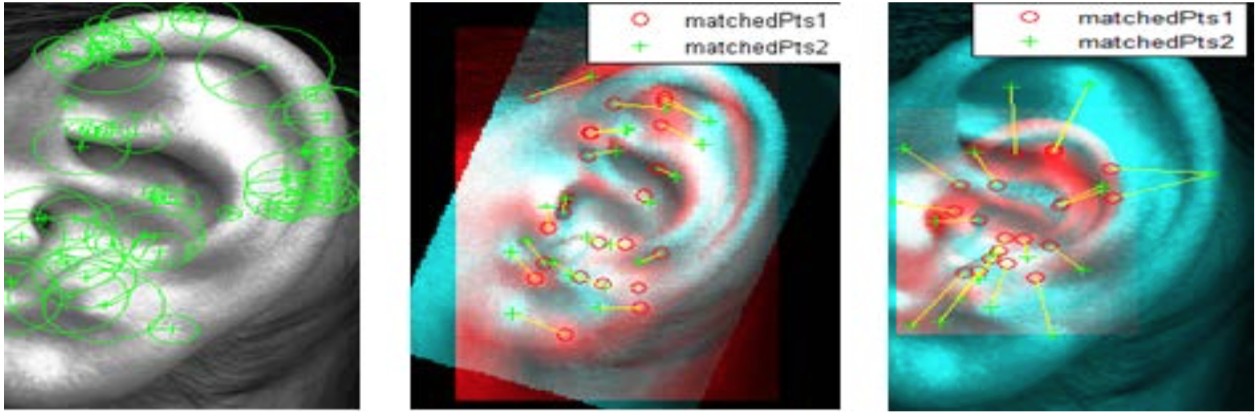
\includegraphics[width=\textwidth]{Figures/Figure9}
	\caption{The detected SURF features (left) and matching result under rotation (middle) and scale change (right)}
	\label{fig:Figure9}
\end{figure}

\textbf{Scale Invariant Feature Transform(SIFT) - } The SIFT features are invariant to image scaling and rotation and shown to provide robust matching across a substantial range of affine distortion, change in 3D viewpoint, addition of noise, and change in illumination. Image matching is a fundamental aspect of many problems in computer vision, including object or scene recognition, solving for 3D structure from multiple images, stereo correspondence, and motion tracking. This paper describes image features that have many properties that make them suitable for matching differing images of an object or scene. The features are invariant to image scaling and rotation, and partially invariant to change in illumination and 3D camera viewpoint. They are well localized in both the spatial and frequency domains, reducing the probability of disruption by occlusion, clutter, or noise. Large numbers of features can be extracted from typical images with efficient algorithms. In addition, the features are highly distinctive, which allows a single feature to be correctly matched with high probability against a large database of features, providing a basis for object and scene recognition.
The cost of extracting these features is minimized by taking a cascade filtering approach, in which the more expensive operations are applied only at locations that pass an initial test. 

 The computation stages of SIFT are as follows: \\
Step 1. Scale space extrema detection: The first step is to construct a Gaussian scale over all the locations. It is implemented efficiently by using a difference of Gaussian (DoG) to identify potential interest points. The 2D Gaussian operator G(x,y,σ) is convolved with the input image \textit{I(x,y)}:
\begin{center}
	$L(x,y,\sigma) = G(x,y,\sigma) * I(x,y)$
\end{center}
where the  DoG images are obtained by subtracting the subsequent scales in each octave.
\begin{center}
	$G(x,y,\sigma) = L(x,y,k\sigma) - L(x,y,\sigma)$
\end{center}

Step 2. Accurate keypoint localization: Once a keypoint has been detected, a detailed model is fitted to determine its location and scale. The keypoints are selected based on measures of their stability. Further details can be found in [16]. 

Step 3. Orientation assignment: One or more orientations are assigned to each key- point location based on local image gradient directions. All future operations are per- formed on image data that has been transformed relative to the assigned orientation, scale, and location for each feature.

Step 4. Keypoint descriptor: The local image gradients are measured at selected scale in the region around each keypoint. They are transformed into a certain representation that allows for significant levels of local shape distortion and shape illumination.

Figure \ref{fig:test4} shows an evaluation of the SIFT detector. It is evident the SIFT keypoints are very stable when the images are rotated and scaled. The scaling results are much better compared to the rotation results in our experiments.
\begin{figure}
\centering
\begin{subfigure}{.5\textwidth}
  \centering
  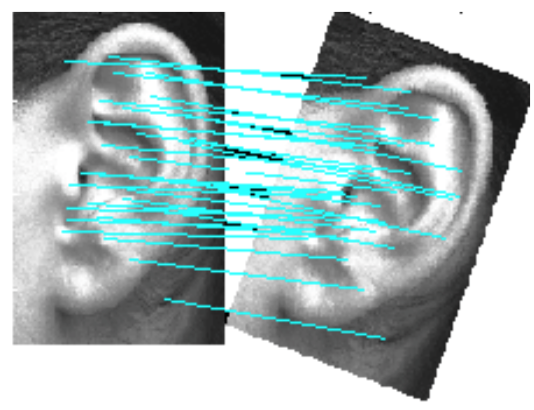
\includegraphics[width=.5\linewidth]{Figures/Figure11}
  \label{fig:sub11}
\end{subfigure}%
\begin{subfigure}{.5\textwidth}
  \centering
  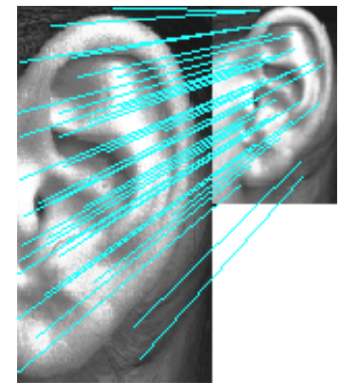
\includegraphics[width=.5\linewidth]{Figures/Figure12}
  \label{fig:sub12}
\end{subfigure}
\caption{The matching results of SIFT detectors under rotation (left) and scale change (right)}
\label{fig:test4}
\end{figure}
